\documentclass[compress,handout,10pt]{beamer}

\newlength{\wideitemsep}
\setlength{\wideitemsep}{\itemsep}
\addtolength{\wideitemsep}{100pt}
\let\olditem\item
\renewcommand{\item}{\setlength{\itemsep}{0.5\baselineskip}\olditem}

\usetheme{Singapore}
\usecolortheme{lily}
\usefonttheme[onlymath]{serif}

\usepackage{float}
\floatstyle{boxed}
\usepackage{colortbl}
\usepackage{mathpazo}
\usepackage{graphicx}
\usepackage{movie15}
\usepackage{bm}
\usepackage{verbatim}
\usepackage{comment}
\usepackage{caption}
\usepackage{subcaption}
\captionsetup[subfigure]{labelformat=empty}
\captionsetup[figure]{labelformat=empty}
\graphicspath{{./Extra/}}

\newcommand{\mygreen}{\color{green!50!black}}
\newcommand{\myblue}{\color{blue}}
\newcommand{\myred}{\color{red}}
\newcommand{\mycolor}{\color{red}{c}\color{blue}{o}\color{green}{l}\color{orange}{o}\color{cyan}{r}}
\newcommand{\mysize}{\scriptsize{s}\small{i}\normalsize{z}\Large{e}}
\newcommand{\myshape}{\textcircled{s}\textit{h}\texttt{a}\textsf{p}\textsc{e}}

\xdefinecolor{titlecolor}{rgb}{.855,.647,.125}
\setbeamercolor{frametitle}{fg=titlecolor}
\setbeamerfont{frametitle}{series=\bfseries}
\setbeamercolor{normal text in math text}{parent=math text}

\setbeamertemplate{navigation symbols}{} %gets rid of navigation symbols
\setbeamertemplate{footline}[frame number]
\beamertemplateshadingbackground{blue!5}{yellow!10}

\title{{\color{blue} \LARGE How much Ice do You need?\newline} }

\subtitle{{\color{red} \large Final Presentation} }

\author{ 
%    \vspace{5pt}
    {\bf{Participants:}} \\ 
Joyce Tan \\ 
Yen Theng Tan \\
    \vspace{5pt}
} 
\institute{JHU AMS 2012 FALL}

\date{\mygreen Last Complied on November 27, 2012} 
\graphicspath{{./extra/}}
\begin{document}

\begin{frame}[plain]
    \titlepage
\end{frame}


\begin{frame}
    \frametitle{Outline}
      \tableofcontents
\end{frame}

\section{Introduction}
\subsection{Sponsor}
\begin{frame}
    \frametitle{Sponsor: McDonald's Corporation}
    \begin{itemize}
     \item McDonald's Corporation is the world's largest chain of hamburger fastfood restaurants, serving around 68 million customers daily in 119 countries.
\item Mcdonald's primarily sells hamburgers, cheeseburgers, chicken, French fries, breakfast items, soft drinks, milkshakes and desserts. 
    \end{itemize}
\end{frame}

\begin{frame}
    \frametitle{Sponsor: McDonald's Corporation}
    \begin{itemize}
         	\item In response to healthier consumer taste, the company has expanded its menu to include salads, wraps, smoothies and fruits.
	 \item No meal is complete without a drink; and from Diet Coke to low-fat milk to fresh-brewed, hot coffee, McDonald's serves many different varieties of beverages
    \end{itemize}
\end{frame}

\subsection{Problem Statement}
\begin{frame}
    \frametitle{Problem Statement}
     \begin{itemize}
         \item Selling soft drinks is a complement to any meal that a customer purchases at McDonald's.
\item However, the server is not accustomed to putting much thought in measuring the amount of ice put in the cup.
\item This often results in a overly diluted, or overly cold drink for the customer. This is likely to lower overall customer satisfaction, since a drink is a significant complement to a meal. 
\item Thus, customers are likely to appreciate if the right amount of ice was added for optimal satisfaction.
     \end{itemize}
\end{frame}

\begin{frame}
    \frametitle{Problem Statement}
     \begin{itemize}
      \item To further define this problem, the exogenous variables are the proportion of ice to put in a drink. 
\item The endogenous variable would be the resulting temperature and concentration of the drink, as we are assuming that a customer's satisfaction is affected only by the temperature and concentration of the drink.
     \end{itemize}
\end{frame}

\subsection{Deliverables}
\begin{frame}
    \frametitle{Deliverables - From Team to Sponsor}


\begin{itemize}
    \item A table of optimal ice proportions/ratios for each different type of soda (namely Coca Cola, Sprite, Fanta Orange, Diet Coke),
    \item Matlab code with complete set of documentations that resulting temperature and dilution based on specific heat capacities and ice proportions,
    \item Numerical experiment results reporting success rate of different ice proportions,
    \item Technical report and presentations summarizing the work. 
\end{itemize}


\end{frame}

\begin{frame}
    \frametitle{Deliverables - From Sponsor to Team}

\begin{itemize}
    \item Sufficient supply of the 4 different sodas we are concentrating on,
\item Sufficient supply of cups used by McDonald's
    \item Computing resources,
    \item Timely responses to inquiries.
\end{itemize}
\end{frame}

\subsection{Timeline}
\begin{frame}
    \frametitle{Timeline}
\begin{itemize}
    \item Work Statement due date, Sep 28, 2012,
    \item Midterm Presentation due date, Oct 17, 2012,
    \item Progress Report due date, Oct 26, 2012,
    \item Final Presentation due date, Nov 28, 2012,
    \item Final Report due date, Dec 3, 2012.
\end{itemize}
\vspace{6pt} Most of the experiments and coding have been done from mid-October to mid-November.
\end{frame}

\section{Content}
\subsection{Approach Assumptions}
\begin{frame}
    \frametitle{Approach Assumptions}

\begin {itemize}
\item Consumer's taste depends entirely on the dilution and temperature factors.
\item Dilution and temperature of drink come hand-in-hand and rely entirely on the ice proportion.
\item Sample group accurately represents the population's preferred combinations of temperature and dilution.
\item The different time parameters which we perform the experiment is sufficient to represent the overall satisfaction the customer has with the drink.
\end{itemize}
\end{frame}

\subsection{Experimental Approach}
\begin{frame}
    \frametitle{Approach 1: Experimental}

\begin {itemize}
\item Experimenting with different types of soda - namely  McDonald's Coca Cola, Sprite, Fanta Orange, and Diet Coke.
\item By experiment, we will test out which ice proportion will yield the highest satisfaction from the test subjects.
\end{itemize}

\end{frame}

\begin{frame}
    \frametitle{Approach 1: Experimental}

\begin {itemize}

\item We will provide 3 different cups of the same soda (different ice proportions) for the test subject to drink and they will indicate their preference. 
\item The ice will be left in the drink for a time period of t (t=0.5mins, 2 mins, 5 mins, 30 mins). The different experiments for the time parameters will be spaced an hour apart.
\item This will be repeated for 3 more days for the other 3 drinks.
\end{itemize}
\end{frame}

\begin{frame}
    \frametitle{Approach 1: Experimental}

\begin {itemize}

\item This will be a blind test and the subject will not know what ice proportions the cups A, B, C have.
\end{itemize}
\vspace{6pt}

\begin{table}[ h]
\centering
\begin{tabular}{ l | c|c|c }
  Ice Proportion & A  & B & C  \\
\hline  
t=0.5mins & & &\\ 
\hline  
t=2mins & & &\\ 
\hline  
t=5mins  & & &\\ 
\hline  
t=30mins & & &\\ 
\hline  
   
 \end{tabular}
\caption{Sample form each test subject will need to fill out for each drink}

\end{table}

\end{frame}

\begin{frame}
    \frametitle{Approach 1: Experimental}

\begin {itemize}

\item Subject will be required to rank preference of the labelled cups for each time parameter t (3 is most favorite).
\end{itemize}
\vspace{6pt}

\begin{table}[ h]
\centering
\begin{tabular}{ l | c|c|c }
  Ice Proportion & A  & B & C  \\
\hline  
t=0.5mins & 3&2 &1\\ 
\hline  
t=2mins &1 &3 &2\\ 
\hline  
t=5mins  &2 &3 &1\\ 
\hline  
t=30mins &1 &2 &3\\ 
\hline  
   
 \end{tabular}
\caption{Example of a response}

\end{table}

\end{frame}


\subsection{Physics-based Approach}
\begin{frame}
    \frametitle{Approach 2: Physics-based}

\begin {itemize}
\item Utilizing the specific heat capacities of soda and ice (already found as specific values), we can calculate the different temperatures and dilution that the resulting drink will have.

\item This will be used mainly as a support tool since it's just mathematical calculation, to see how much ice proportion actually affects dilution as well as resulting temperature
\end{itemize}

\end{frame}

\subsection{Results}
\begin{frame}
    \frametitle{Results - Experimental approach}

\begin{table}[ h]
\centering
\begin{tabular}{ l || c|c|c }
  &40\% &60\% & 75\%  \\
\hline  
t=0.5 mins & 15 & 25 & 32\\ 
\hline  
t=2 mins & 14 & 24 & 34\\ 
\hline  
t=5 mins & 14 & 27 & 31\\ 
\hline  
t=30 mins & 18 & 36 & 18\\ 
\hline  
   
 \end{tabular}

\caption{Experiment results for Coke}

\end{table}
\end{frame}

\begin{frame}
    \frametitle{Results - Experimental approach}

\begin{table}[ h]
\centering
\begin{tabular}{ l || c|c|c }
  &40\% &60\% & 75\%  \\
\hline  
t=0.5 mins & 15 & 27 & 30\\ 
\hline  
t=2 mins & 20 & 19 & 33\\ 
\hline  
t=5 mins & 14 & 29 & 29\\ 
\hline  
t=30 mins & 17 & 30 & 25\\ 
\hline  
   
 \end{tabular}

\caption{Experiment results for Sprite}

\end{table}
\end{frame}

\begin{frame}
    \frametitle{Results - Experimental approach}

\begin{table}[ h]
\centering
\begin{tabular}{ l || c|c|c }
  &40\% &60\% & 75\% \\
\hline  
t=0.5 mins & 15 & 23 & 34\\ 
\hline  
t=2 mins & 19 & 23 & 30\\ 
\hline  
t=5 mins & 18 & 27 & 27\\ 
\hline  
t=30 mins & 12 & 35 & 25\\ 
\hline  
   
 \end{tabular}

\caption{Experiment results for Fanta Orange}

\end{table}
\end{frame}

\begin{frame}
    \frametitle{Results - Experimental approach}
\begin{table}[ h]
\centering
\begin{tabular}{ l || c|c|c}
  &40\% &60\% & 75\%  \\
\hline  
t=0.5 mins & 15 & 24 & 33\\ 
\hline  
t=2 mins & 21& 19 & 32\\ 
\hline  
t=5 mins & 16 & 24 & 32\\ 
\hline  
t=30 mins & 18 & 22& 32\\ 
\hline  
   
 \end{tabular}

\caption{Experiment results for Diet Coke}

\end{table}
\end{frame}

\begin{frame}
    \frametitle{Results - Physics-based approach}
\begin{table}[ h]
\centering
\begin{tabular}{ l || c|c}
 Volume of ice to volume of soda &Dilution &Temperature (Celsius) \\
\hline  
1/10 & 0.09&16.2\\ 
\hline  
1/8 & 0.11&14.3\\ 
\hline 
1/6 & 0.15&11.2\\ 
\hline 
1/5 & 0.18&8.8\\ 
\hline 
1/4 & 0.23&5.5\\ 
\hline 
   
 \end{tabular}

\caption{Calculated dilution and temperature for difference ice volumes}

\end{table}
\end{frame}
 
\subsection{Analysis}

%% SLIDE 20 onwards - 
% COKE
\begin{frame}
    \frametitle{Analysis - Experimental approach}
\begin{table}[ h]
\centering
\begin{tabular}{ l || c|c|c||c|c }
  &40\% &60\% & 75\% &p-value &significance? \\
\hline  
t=0.5 mins & 15 & 25 & 32 & 0.047&significant\\ 
\hline  
t=2 mins & 14 & 24 & 34&0.016&significant\\ 
\hline  
t=5 mins & 14 & 27 & 31&0.037&significant\\ 
\hline  
t=30 mins & 18 & 36 & 18&0.011&significant\\ 
\hline
Sum of significant rows & 61 & 112 & 115 & & \\ 
\hline     
 \end{tabular}
\caption{Experiment results for Coke}
\end{table}

\begin{itemize}
\item 'Good' set of data, given that the data set are all considered significant by the Chi-Squared Test
\item As time elapses, subjects tend to choose the cup with less ice, but not the least ice
\end{itemize}
\end{frame}


%% SPRITE
\begin{frame}
    \frametitle{Analysis - Experimental approach}
\begin{table}[ h]
\centering
\begin{tabular}{ l || c|c|c||c|c }
  &40\% &60\% & 75\% &p-value &significance? \\
\hline  
t=0.5 mins & 15 & 27 & 30&0.072&not significant\\ 
\hline  
t=2 mins & 20 & 19 & 33&0.079&not significant\\ 
\hline  
t=5 mins & 14 & 29 & 29&0.044&significant\\ 
\hline  
t=30 mins & 17 & 30 & 25&0.011&significant\\ 
\hline  
Sum of significant rows & 31 & 59 & 54 & & \\ 
\hline     

 \end{tabular}
\caption{Experiment results for Sprite}
\end{table}

\begin{itemize}
\item The p-values for t=0.5 mins and t = 2 mins are marginally above 0.05, but is still considered insignificant
\item Ignoring those row of values, we see that at t = 5 mins and t = 30 mins, there is a strong preference towards 60\% and 75\%
\end{itemize}
\end{frame}

%% FANTA ORANGE
\begin{frame}
    \frametitle{Analysis - Experimental approach}
\begin{table}[ h]
\centering
\begin{tabular}{ l || c|c|c||c|c }
  &40\% &60\% & 75\% &p-value &significance? \\
\hline  
t=0.5 mins & 15 & 23 & 34&0.022&significant\\ 
\hline  
t=2 mins & 19 & 23 & 30&0.275&not significant\\ 
\hline  
t=5 mins & 18 & 27 & 27&0.325&not significant\\ 
\hline  
t=30 mins & 12 & 35 & 25&0.004&significant\\ 
\hline     
Sum of significant rows & 27 & 58 & 59 & & \\ 
\hline     
 \end{tabular}
\caption{Experiment results for Fanta Orange}

\end{table}

\begin{itemize}
\item P-values for t = 2 mins and t = 5 mins are quite significantly above our accepted significance levels
\item t = 30 has a very low p-value, indicating a strong lack of randomness
\end{itemize}
\end{frame}

%% DIET COKE
\begin{frame}
    \frametitle{Analysis - Experimental approach}
\begin{table}[ h]
\centering
\begin{tabular}{ l || c|c|c||c|c }
  &40\% &60\% & 75\% &p-value &significance? \\
\hline  
t=0.5 mins & 15 & 24 & 33&0.034&significant\\ 
\hline  
t=2 mins & 21& 19 & 32&0.130 &not significant\\ 
\hline  
t=5 mins & 16 & 24 & 32&0.069&not significant\\ 
\hline  
t=30 mins & 18 & 22& 32&0.115&not significant\\ 
\hline  
Sum of significant rows & 15 & 24 & 33 & & \\ 
\hline     
 \end{tabular}
\caption{Experiment results for Diet Coke}
\end{table}

\begin{itemize}
\item There is much more 'randomness' in this set of data
\item Diet Coke's effect on ice/melting points?
\end{itemize}
\end{frame}

%% TOTAL 
\begin{frame}
    \frametitle{Analysis - Experimental approach}
\begin{table}[ h]
\centering
\begin{tabular}{ l || c|c|c }
  &40\% &60\% & 75\%  \\
\hline  
Coke & 61 & 112 & 115 \\
\hline  
Sprite & 31& 59 & 54 \\
\hline  
Fanta Orange & 27 & 58 & 59 \\ 
\hline  
Diet Coke & 15 & 24& 33 \\ 
\hline  
Total & 134 & 253 & 261  \\ 
\hline     
 \end{tabular}
\caption{Experimental Totals}
\end{table}

\begin{itemize}
\item Taking the significant sets of data into consideration, there is an overall tendency for our subjects to prefer the 60\% and 75\% choices

\end{itemize}

\end{frame}


%% ANALYSIS 
\begin{frame}
    \frametitle{Analysis - Physics-based approach}
\begin{table}[ h]
\centering
\begin{tabular}{ l || c|c}
 Volume of ice to volume of soda &Dilution &Temperature (Celsius) \\
\hline  
1/10 & 0.09&16.2\\ 
\hline  
1/8 & 0.11&14.3\\ 
\hline 
1/6 & 0.15&11.2\\ 
\hline 
1/5 & 0.18&8.8\\ 
\hline 
1/4 & 0.23&5.5\\ 
\hline    
\end{tabular}
\caption{Calculated dilution and temperature for difference ice volumes}
\end{table}

\begin{itemize}
\item Dilution / Temperature equilibrium 
\end{itemize}

\end{frame}

%% GRAPH 
\begin{frame}
    \frametitle{Analysis - Physics-based approach}

\begin{figure}
	\centering
	\caption{Graph of Dilution and Temperature against different ice volumes}
	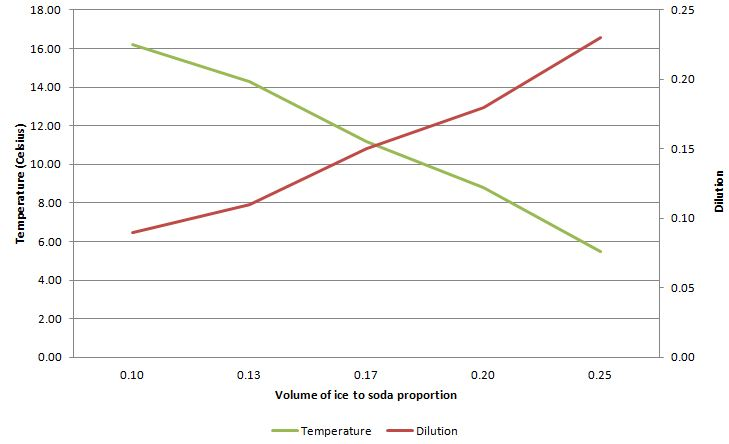
\includegraphics[width=\textwidth]{Extra/Graph.jpg}
\end{figure}

\end{frame}


%%%%%%% CONCLUSION %%%%%%%%

% From Team to Sponsor
\section{Conclusion}
\subsection{Deliverables}
\begin{frame}
    \frametitle{Deliverables - From Team to Sponsor}


\begin{itemize}
    \item A table of optimal ice proportions/ratios for each different type of soda (namely Coca Cola, Sprite, Fanta Orange, Diet Coke),
    \item Matlab code with a complete set of documentations that show the resulting temperature and dilution calculations based on specific heat capacities and ice proportions,
    \item Numerical experiment results (raw data) of subject's preferences,
    \item Technical report and presentations summarizing our work. 
\end{itemize}


\end{frame}

\begin{frame}
    \frametitle{Deliverables - From Sponsor to Team}

\begin{itemize}
    \item Sufficient supply of the 4 different sodas we are working with on,
\item Sufficient supply of cups used by McDonald's
    \item Computing resources,
    \item Timely responses to inquiries.
\end{itemize}
\end{frame}

%% Advantages and Disadvantages
\subsection{Advantages and Disadvantages}

%Advantages
\begin{frame}
    \frametitle{Advantages}

\begin {itemize}
\item Comprehensive study of consumer preferences, factoring in time, as opposed to arbitrary ice-filling.
\item Utilizing the specific heat capacities of soda and ice, we can calculate the different desired combinations of temperatures and dilution of the drink.
\item Good foundation for further studies with larger populations and additional factors
\end{itemize}

\end{frame}

%Disadvantages 
\begin{frame}
    \frametitle{Disadvantages}

\begin{itemize}
\item Different consumer tastes regarding temperature and dilution. 
\item Desired temperature of drink is likely to vary with location.
\item Different types of Soda may have differing effects on ice and their melting points
\item Physics-based calculation assumes no inteference with the environment
\end{itemize}

\end{frame}
 

%Further Recommendations
\subsection{Further Recommendations}
\begin{frame}
    \frametitle{Further Recommendations}
\begin{itemize}
\item Perform experiments on different days with different climates.
\item Larger subject population
\item Specificity in project objectives 
\item Split sample group based on gender and age.
\end{itemize}
\end{frame}

\begin{frame}[plain]
    \titlepage
\end{frame}

\end{document}
